


En este capítulo se expone la planificación de tareas que se ha seguido para desarrollar \nombrejuego{}. En primer lugar se adjunta el diagrama de Gantt completo para, más adelante, complementarlo con un breve comentario de cada tarea.

\section{Diagrama de Gantt}
Como puede observarse en el diagrama de Gantt, en el apartado artístico de \nombrejuego{} participan más personas. Esto se debe a que no poseía ni poseo los conocimientos o destrezas requeridos para crear modelos 2D y sus animaciones, escenarios de la ciudad de Cádiz, todo en \cursiva{pixel art}, piezas musicales, efectos de sonido ni un guión de diálogos y descripciones completo con su correspondiente traducción al inglés. Por ello, he contactado con gente con experiencia en dichas materias dispuestos a colaborar en el desarrollo de un videojuego completamente libre. Además de una persona que asesore en el área histórica del videojuego para evitar incongruencias. Finalmente, los participantes adicionales son:

\begin{itemize}
\item Celia Fermoselle: artista especializada en\cursiva{pixel art} encargada de diseñar, dibujar, animar a los personajes, objetos y escenarios del juego.
\item boredBit: grupo formado por Dmitry Jbanov y Manu Garrido que se encargan de componer y producir la banda sonora completa y efectos de sonido para el juego.
\item Daniel Brey: encargado de escribir en su mayoría del guión de diálogos y descripciones del juego.
\item Laura J. Torres: encargada en traducir el guión del juego del español al inglés.
\item Encarnación M. R. : encargada en asesorar el contenido histórico del proyecto para evitar incongruencias.
\end{itemize}

El diagrama de Gantt sobre la planificación del proyecto es el siguiente:

\begin{figure}[H] 
  \begin{center}
    %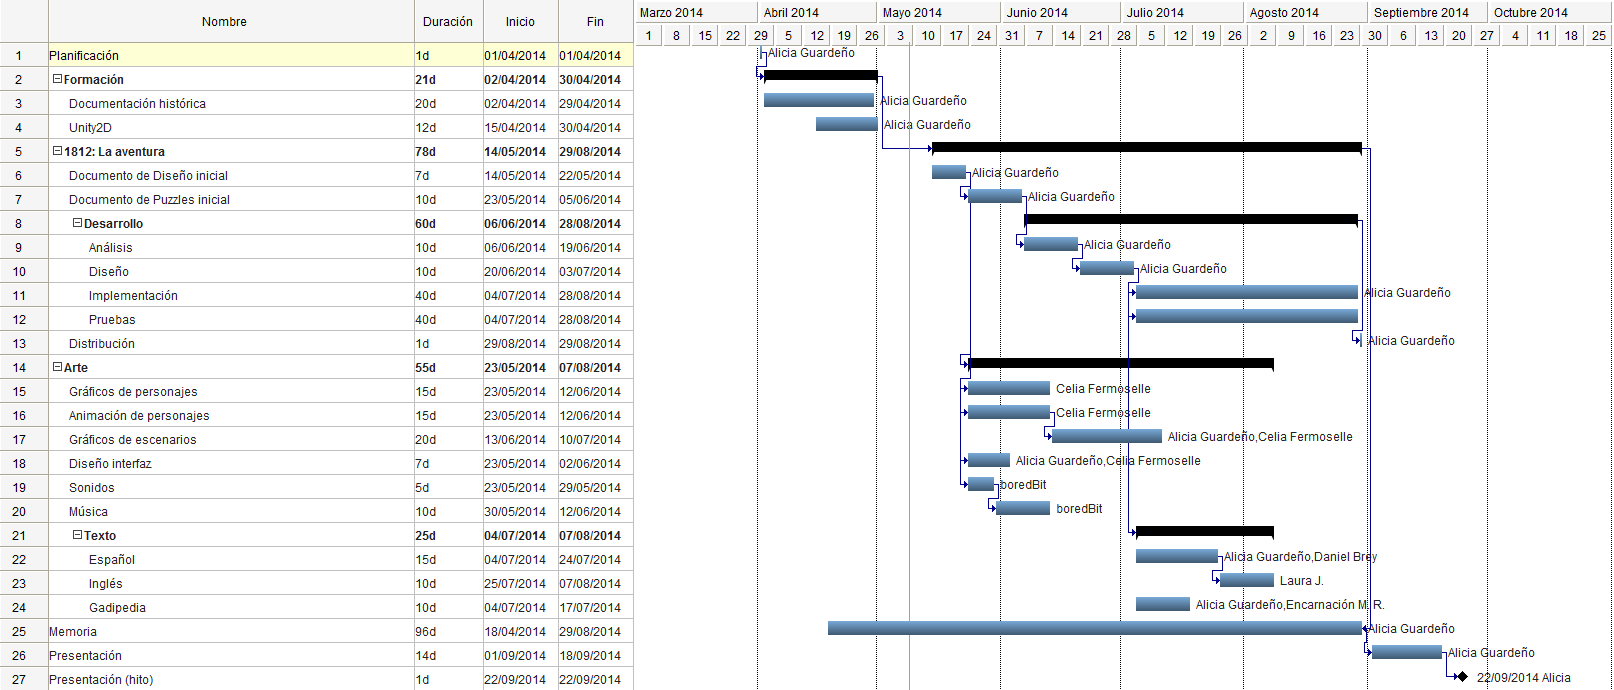
\includegraphics[scale=0.4]{planificacionv2-1.png}
    \makebox[\textwidth]{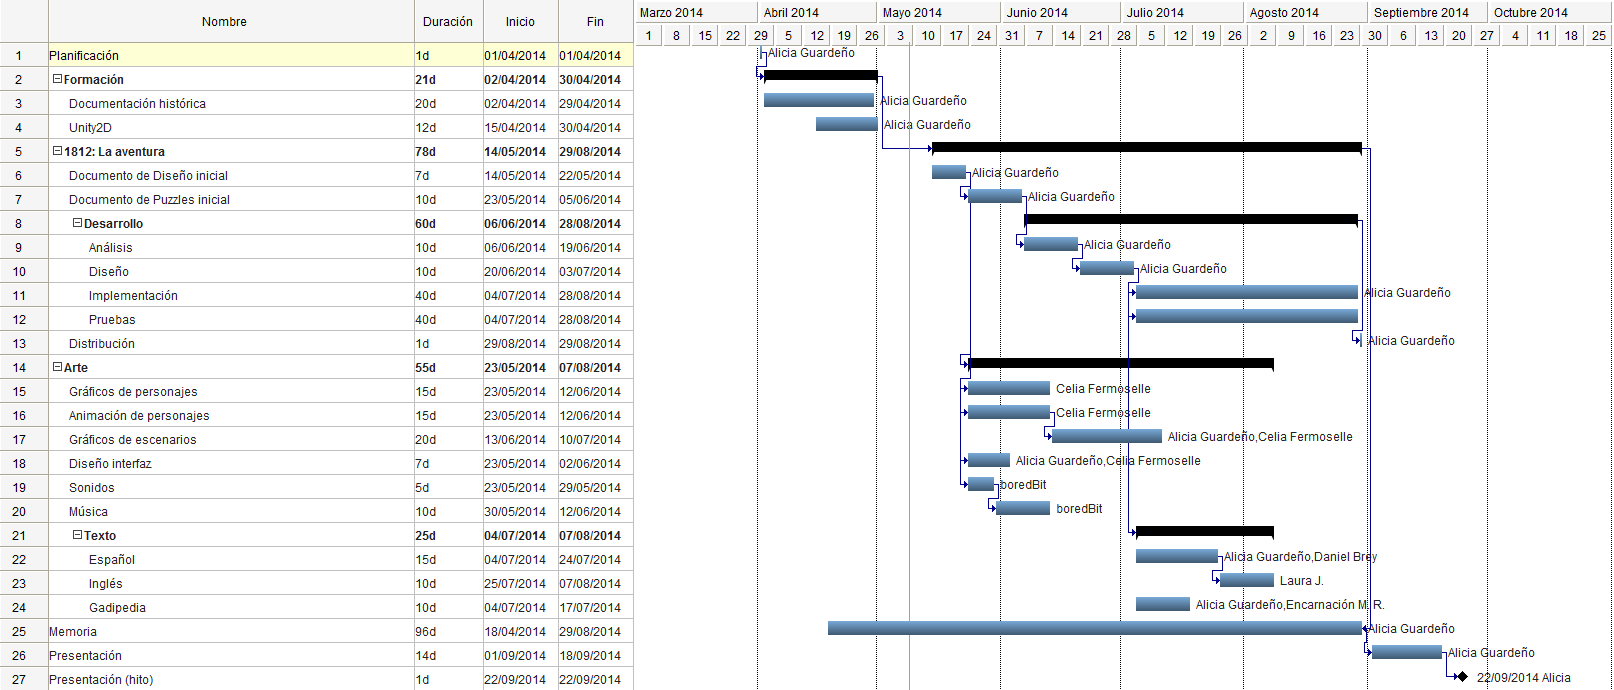
\includegraphics[width=0.9\paperwidth]{planificacionv2-1.png}}
  \end{center}
  \caption{Planificación del proyecto desde abril de 2014 hasta septiembre de 2014}
    \label{fig:gantt}
\end{figure}

\section{Etapas de desarrollo del proyecto}

\begin{enumerate}
\item\negrita{Planificación} \hfill \\
Dada la envergadura del proyecto, era necesaria una etapa de planificación en la que se ha estudiado de forma cuidadosa el alcance del mismo y las posibles dificultades a encontrar durante el desarrollo.

\item\negrita{Formación} \hfill \\
Al comienzo del proyecto desconocía por completo el uso de \programa{Unity3D} y su API, el lenguaje C\#. Además de carecer de conocimientos históricos profundos sobre el Cádiz en la época de 1812. Fue necesaria, por tanto, una larga etapa de formación personal utilizando varios recursos bibliográficos, tanto históricos como para desarrollo de videojuegos, y pequeñas pruebas prácticas en \programa{Unity3D}.

\item\negrita{1812: La aventura} \hfill \\
Tras el periodo de aprendizaje, se comenzó con el videojuego \nombrejuego{}. El primer paso fue crear una cuenta en la forja de \programa{GitHub}. Dicha forja proporciona un repositorio \emph{Git} y herramientas web que ayudan en la gestión de un proyecto: gestor de tareas, subida de ficheros, publicación de noticias, wiki, foros, etc.

\begin{enumerate}
\item \emph{Documento de diseño} \hfill \\
En el documento de diseño de un videojuego se detallan elementos como la historia, género, personajes, mecánicas de juego, objetos o escenarios entre otros muchos. En definitiva, es el documento que define de forma más o menos concisa cómo será el videojuego. Se trata de un escrito muy importante ya que ayuda a que todo el equipo albergue la misma idea sobre el videojuego y pueda trabajar de forma más compenetrada.

\item \emph{Documento de puzzles} \hfill \\
En el documento de puzzles de un videojuego, más propiamente de una aventura gráfica, en la que se detallas los puzzles, la jerarquía de resolución de puzzles, escenarios y objetos involucrados en su resolución. Se trata de un escrito muy importante ya que determina el flujo del desarrollo de una aventura gráfica, y lo entretenido que pueda llegar a ser para un usuario.

\item \emph{Análisis} \hfill \\
La fase de análisis dió comienzo después de la redacción y revisión de los documentos de diseño y puzzles. Se procedió con la toma de requisitos a partir de dicho documento, se confeccionaron los casos de uso, se elaboró el modelo conceptual de datos y se detalló el modelo de comportamiento.

\item \emph{Diseño} \hfill \\
Durante la fase de diseño, que siguió de forma inmediata al análisis, se elaboraron los diagramas de clases.

\item \emph{Implementación} \hfill \\
La fase de implementación de \nombrejuego{} fue, con diferencia, la más extendida de todo el desarrollo. Quizás viniese motivada por la inexperiencia y los varios sistemas, entre ellos una pequeña base de datos,  que se tuvieron que implementar desde la base.

\item \emph{Pruebas} \hfill \\
Durante la implementación se fueron realizando pruebas de módulos individuales pero fue tras finalizar dicha fase cuando tuvieron lugar las pruebas de integración. No sólo se trabajó para que el código fuese correcto, sino que \nombrejuego{} fue probado de forma extensiva por colaboradores distintos al desarrollador principal con el claro objetivo de pulir ciertos detalles relacionados como el balanceo de la dificultad de los puzzles (que no sean ni fáciles ni difíciles), el correcto control del personaje entre otras cosas.

%\item \emph{Mantenimiento} \hfill \\
%

\item \emph{Distribución} \hfill \\
Se crearon y publicaron paquetes descargables para los sistemas GNU/Linux, MacOSX y Windows. Por suerte \programa{Unity3D} es un editor que cuenta con un compilador multiplataforma, con lo que solo tomó un día en crear todos los paquetes.  
%

\item \emph{Arte} \hfill \\
El proceso de creación la mayor parte del arte necesario para \nombrejuego{} comenzó nada más acabar la redacción del documento de diseño, exceptuándo algunas partes del guión que eran dependientes de la finalización del documento de puzzles. Desde el momento que se tenía completado el documento de diseño, se conocía el estilo visual del juego, los escenarios, personajes y música que aparecerían. Por su complejidad, el trabajo se extendió prácticamente durante todo el desarrollo. Al ser la única tarea en la que participaron colaboradores, fueron necesarias labores de supervisión y coordinación: estilo, formato de entrega, corrección de fallos, etc.

\begin{enumerate}
\item \emph{Gráficos de personajes} \hfill \\
Los gráficos los realizó Celia Fermoselle, realizados con la técnica de \cursiva{pixel art} dado que era como mejor y más rápido trabajaba. La coordinación en este punto fue crítica pues había que llegar a una estética que gustase al público y que a su vez fuera sencillo de realizar.

\item \emph{Animación de personajes} \hfill \\
Una vez finalizados los gráficos de los personajes, Celia tuvo que hacer su animación por cuadros. Esta técnica se basa en modificar los gráficos originales en sucesivos cuadros, que al repetirse rápidamente dan ilusión de movimiento. Teniendo el estilo ya definido de los primeros gráficos, la supervisión y coordinación no fue tan cargante.

\item \emph{Gráficos de escenarios} \hfill \\
Aquí el trabajo fue realizado por un grupo: Celia se encargaba de realizar los escenarios en \cursiva{pixel art}, mientras tanto, yo le pasaba fotos de escenarios reales en los que basarse y los bocetos de los escenarios ficticios a partir de las fotos. Para poder realizar las fotos, fue necesaria la ayuda de [...], perteneciente a la Asociación de Recreación Histórica del Cádiz de 1812, el cual nos facilitó el acceso a trajes, armas, sitios de relevancia de la época, etc.

\item \emph{Diseño de la interfaz} \hfill \\
A partir del documento de diseño, la interfaz fue realizada rápidamente por Celia Fermoselle.

\item \emph{Efectos de sonido} \hfill \\
Una vez detallados los sonidos requeridos en el documento de diseño, estos fueron realizados por el equipo de músicos boredBit.

\item \emph{BSO} \hfill \\
Ya acabados los sonidos principales del juego, boredBit se dispuso a realizar la música del juego. La coordinación fue necesaria, para en el mismo caso que los gráficos, se definiera un estilo de música que fue incluido el documento de diseño.


\item \emph{Texto} \hfill \\
Siendo \nombrejuego{} una aventura gráfica, la calidad de los diálogos y descripciones es necesaria para ser disfrutado por el público y ayudar a la resolución de puzzles. Daniel Brey se prestó a colaborar conmigo para la realización de estos fijándonos en el documento de diseño y de puzzles, también Encarnación M. R. que asesoró que no hubiera incongruencias en los contenidos relacionados con el Cádiz de 1812.

\begin{enumerate}
\item \emph{Español} \hfill \\
Tal y como se ha dicho en el apartado anterior, Daniel Brey realizó el guión del videojuego en español sirviéndose del documento de diseño y puzzles, además de contar con mi ayuda y la de Encarnación M. R. en temas históricos.

\item \emph{Inglés} \hfill \\
Finalizado los textos en español, Laura J. Torres procedió a transcribirlos al inglés. Durante la transcripción, fue necesaria la coordinación para indicarle el formato que tenía que seguir el texto. Posteriormente ayudó en la realización de un documento que dictase los pasos a seguir para modificar los textos o traducirlos a otros idiomas más adelante.

\item \emph{Gadipedia} \hfill \\
La extraña palabra Gadipedia viene a ser una pequeña enciclopedia de los hechos más importantes de la época del Cádiz de 1812, además de incluir algunas anécdotas que nos ayudan a vislumbrar la vida cotidiana de entonces como los uniformes, el comercio, etc. Todo ello accesible desde dentro del juego para ayudar a la resolución de los puzzles. Ahora bien, si la parte de la implementación corrió a cuenta mía, la de la generación y supervisión de los textos fue gracias a Encarnación M. R.

\end{enumerate}

\end{enumerate}

\end{enumerate}

\item\negrita{Memoria} \hfill \\
Antes, durante y después del desarrollo de \nombrejuego{} se procedió a la redacción del presente documento que incluye apéndices adicionales como el manual de usuario del videojuego.

\item\negrita{Presentación} \hfill \\
Como última tarea en la organización temporal figura la elaboración de la exposición de cara a la presentación del \negrita{Proyecto fin de Carrera}. Se llevó a cabo tratando de plasmar el trabajo realizado y los objetivos conseguidos con el desarrollo de este proyecto.

\item\negrita{Comunidad} \hfill \\
Una de las partes fundamentales de este proyecto es su objetivo de servir a la comunidad. Hasta el momento había una escasa documentación sobre cómo diseñar un videojuego en español, más concretamente al diseño de las aventuras gráficas. A lo largo de todo el desarrollo ha estado presente la atención e interacción con la comunidad a través de diversos medios como redes sociales, foros de desarrolladores de videojuegos y el blog.

\item\negrita{Presentación (hito)} \hfill \\
Finalmente, el día [...] se entrega toda la documentación del proyecto y se preparó la presentación final que tendría lugar, aproximadamente, [...] después.

\end{enumerate}
